\chapter{Analysis}
In this chapter we will explain the problem and objectives we're tackling with this work, as well as our requirements and experiments performed.

\section{Problem and objectives}
As discussed in the State of the Art chapter, there are many ways to accelerate a ray tracing application, and not all of them work the same way. When building a ray tracer, it's important to know the differences between the technologies behind this acceleration in order to pick the one that best suits our requirements.

As explained in the Introduction, we have nailed down the two most relevant options to Vulkan and OptiX. Our objective is to analyze how each of them behave when varying the rendering quality and scene complexity.

For our objectives to be met and our experiments to be performed we will need the following:

\begin{itemize}
  \item[*]{Ray Tracer capable of rendering with the Vulkan API and its ray tracing extension and Ray Tracer capable of rendering with the OptiX library, both capable of drawing images as similar as possible. Both renderers may be the same application with some mechanism to switch APIs, but they could also be separate projects with equivalent features. They will also need to be parametrized, so our automation tools can run our experiments from the command line.}
  \item[*]{Set of experiments to run on both renderers. These must test different ammounts of scene geometry and image quality settings, like screen resolution.}
  \item[*]{Automation system to run our set of experiments in a consistent and replicable way.}
  \item[*]{Result visualization system, to plot the results from our experiments.}
\end{itemize}

\section{Experiment Design}
The first step before starting to record any data or implementing any renderers was to decide what kind of experiments we wanted to run. After reading recent publications on the topic of ray and path tracing, we settled for the same measurements done by Nvidia at the last GTC, when they introduced some advances in real-time path tracing \cite{Clarberg2022}. These are frame time, acceleration structure building time, and memory usage.

\begin{figure}[hbt!]
    \centering
    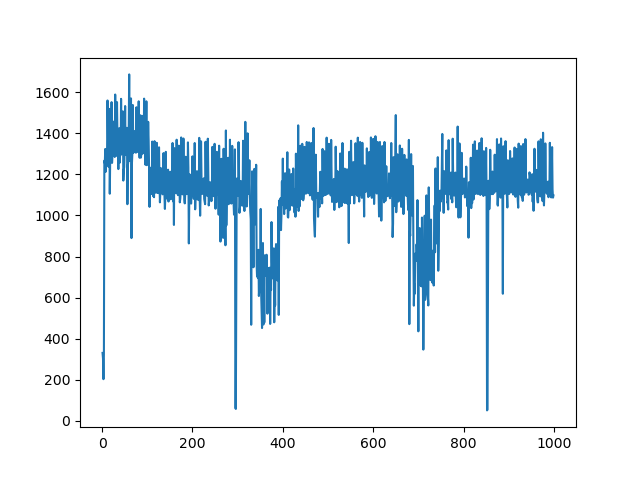
\includegraphics[width=1.0\textwidth]{figuras/vulkan-7680x4320viking_room-textures-frametimes.png}
    \caption{Render times over 1000 frames with a frame buffer resolution of 7680x4320, while drawing the model of a viking room with textures. It can be observed how in a very short span of time, the rendering time of the exact same geometry and effects can hugely change.}
    \label{vulkan-7680x4320viking_room-textures-frametimes}
\end{figure}

\begin{itemize}
    \item[*]\textbf{Acceleration Structure Building Time:} as the name suggests, this is a spatial data structure that speeds up the search for triangles, distance fields and other geometry primitives in a given scene. Ray tracing applications use these to achieve better performance. For example, it's much faster to look for ray intersections by traversing a hierarchical structure of Axis Aligned Bounding Boxes than to check a ray against every triangle in a scene. These structures are typically comprised of a single Top Level Acceleration Structure (TLAS) containing multiple Bottom Level Acceleration Structures (BLAS), which encode a single 3D model each with a 3x4 transformation matrix. These structures are usually implemented in hardware. The time it takes for them to be built can be relevant on the general application's startup time for a static scene such as the ones we will be testing, and for runtime performance in case of scenes with dynamic geometry, where this structure will need to be rebuilt for every animation step.
    \item[*]\textbf{Frame Time:} videogames and the media that traditionally covers them have engraved in the general public the notion that Frames Per Second (FPS) is the most important performance metric in an interactive graphical application. While this is probably true for the end user experience, the FPS count can be affected by a miriad of things outside of the rendering system, such as GPU-CPU synchronization, physics simulation, etc. As this work aims to compare only the rendering performance of each library, we will only be measuring the time it takes to write the rendered images to a frame buffer. Due to the huge variance of running times inside a modern Operating System, the render times can vary wildly as well (as we can see in \ref{vulkan-7680x4320viking_room-textures-frametimes}). To mitigate this, we will take the time measurements over a fairly long period of time (1000 frames) and average them together in order to get a more precise idea of the rendering time that's less subject to flukes.
    \item[*]\textbf{Memory Usage:} quite self-explanatory, the last factor we consider of great importance is the video memory consumption of the process. This can be a limiting factor on the hardware requirements of a particular application, since execeding the user's GPU's memory capabilities will force it to resort to the use of swap memory from the system RAM, significantly impacting the performance due to an abundance of copying between the two.
\end{itemize}

All these variables will be tested while rendering different ammounts of geometry and scene complexity. In order to simplify the development of all renderers, each scene will be comprised of a single 3D model. The Single Triangle model was built in-house, the Viking Room was obtained from \cite{VulkanTutorial}, and the rest were obtained from Morgan McGuire's Computer Graphics Archive \cite{McGuire2022Data}. They all can be seen at table \ref{scenes-geometry-table} and in figures \ref{bmw-screenshot}, \ref{sponza-screenshot} and \ref{hairball-screenshot}.

\begin{center}
  \begin{tabular}{ | m{3cm} | m{3cm}| m{3cm}|m{3cm} |}
  \hline
  Model name& Triangles& Vertices& Texture size\\
  \hline
    Single Triangle& 1& 3& 0\\
  \hline
    Viking Room& 2000& 2600& 0\\
  \hline
    BMW& 385079& 249772& 0\\
  \hline
    Sponza& 262267& 184330& 74.0 MB\\
  \hline
    Hairball& 2880000& 1441098&0\\
  \label{scenes-geometry-table}
\end{tabular}
  % \caption{Scenes that will be used to test the ray tracing libraries compared in this work. We have selected a single 3D model from each order of magnitude in terms of size.}
\end{center}

\begin{figure}[hbt!]
  \centering
  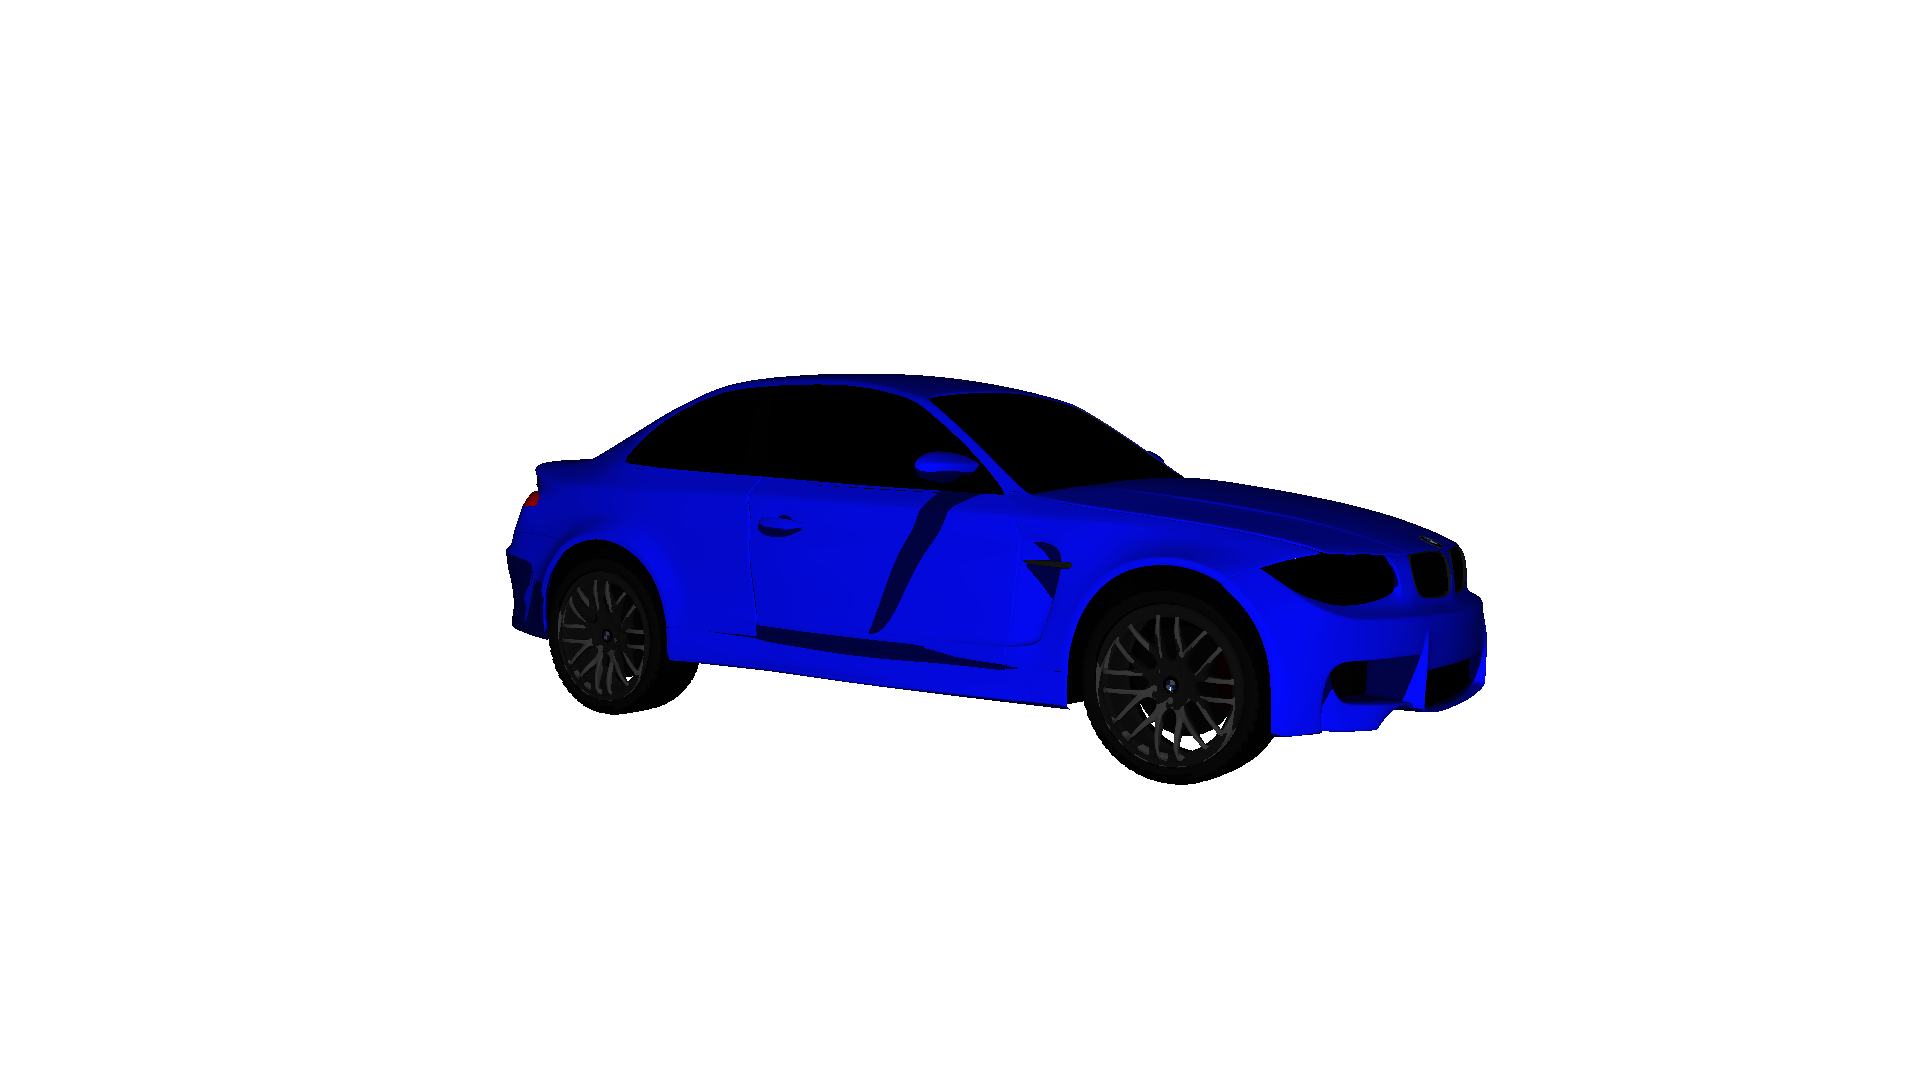
\includegraphics[width=0.75\textwidth]{figuras/bmw.png}
  \caption{BMW 3D model used during our experiments}
  \label{bmw-screenshot}
\end{figure}

\begin{figure}[hbt!]
  \centering
  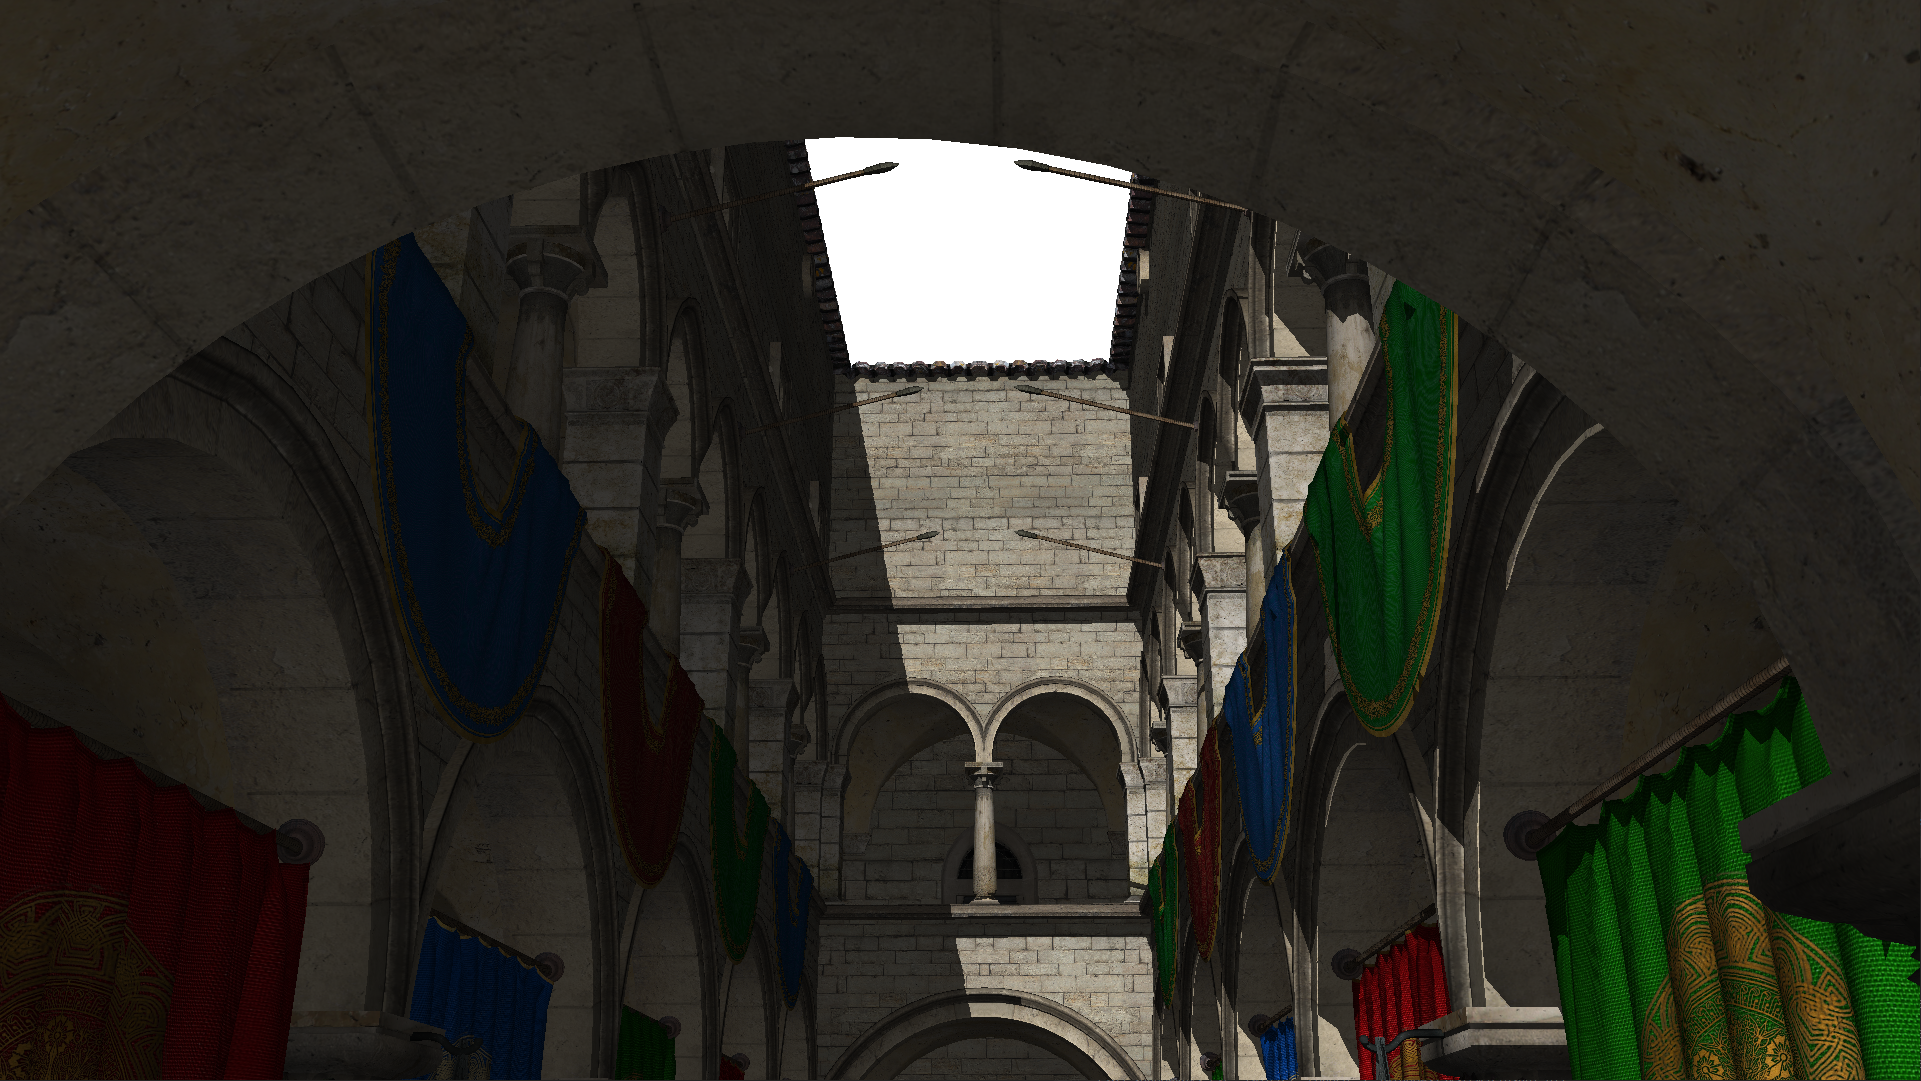
\includegraphics[width=0.75\textwidth]{figuras/sponza.png}
  \caption{Sponza 3D model used during our experiments}
  \label{sponza-screenshot}
\end{figure}
\begin{figure}[hbt!]
  \centering
  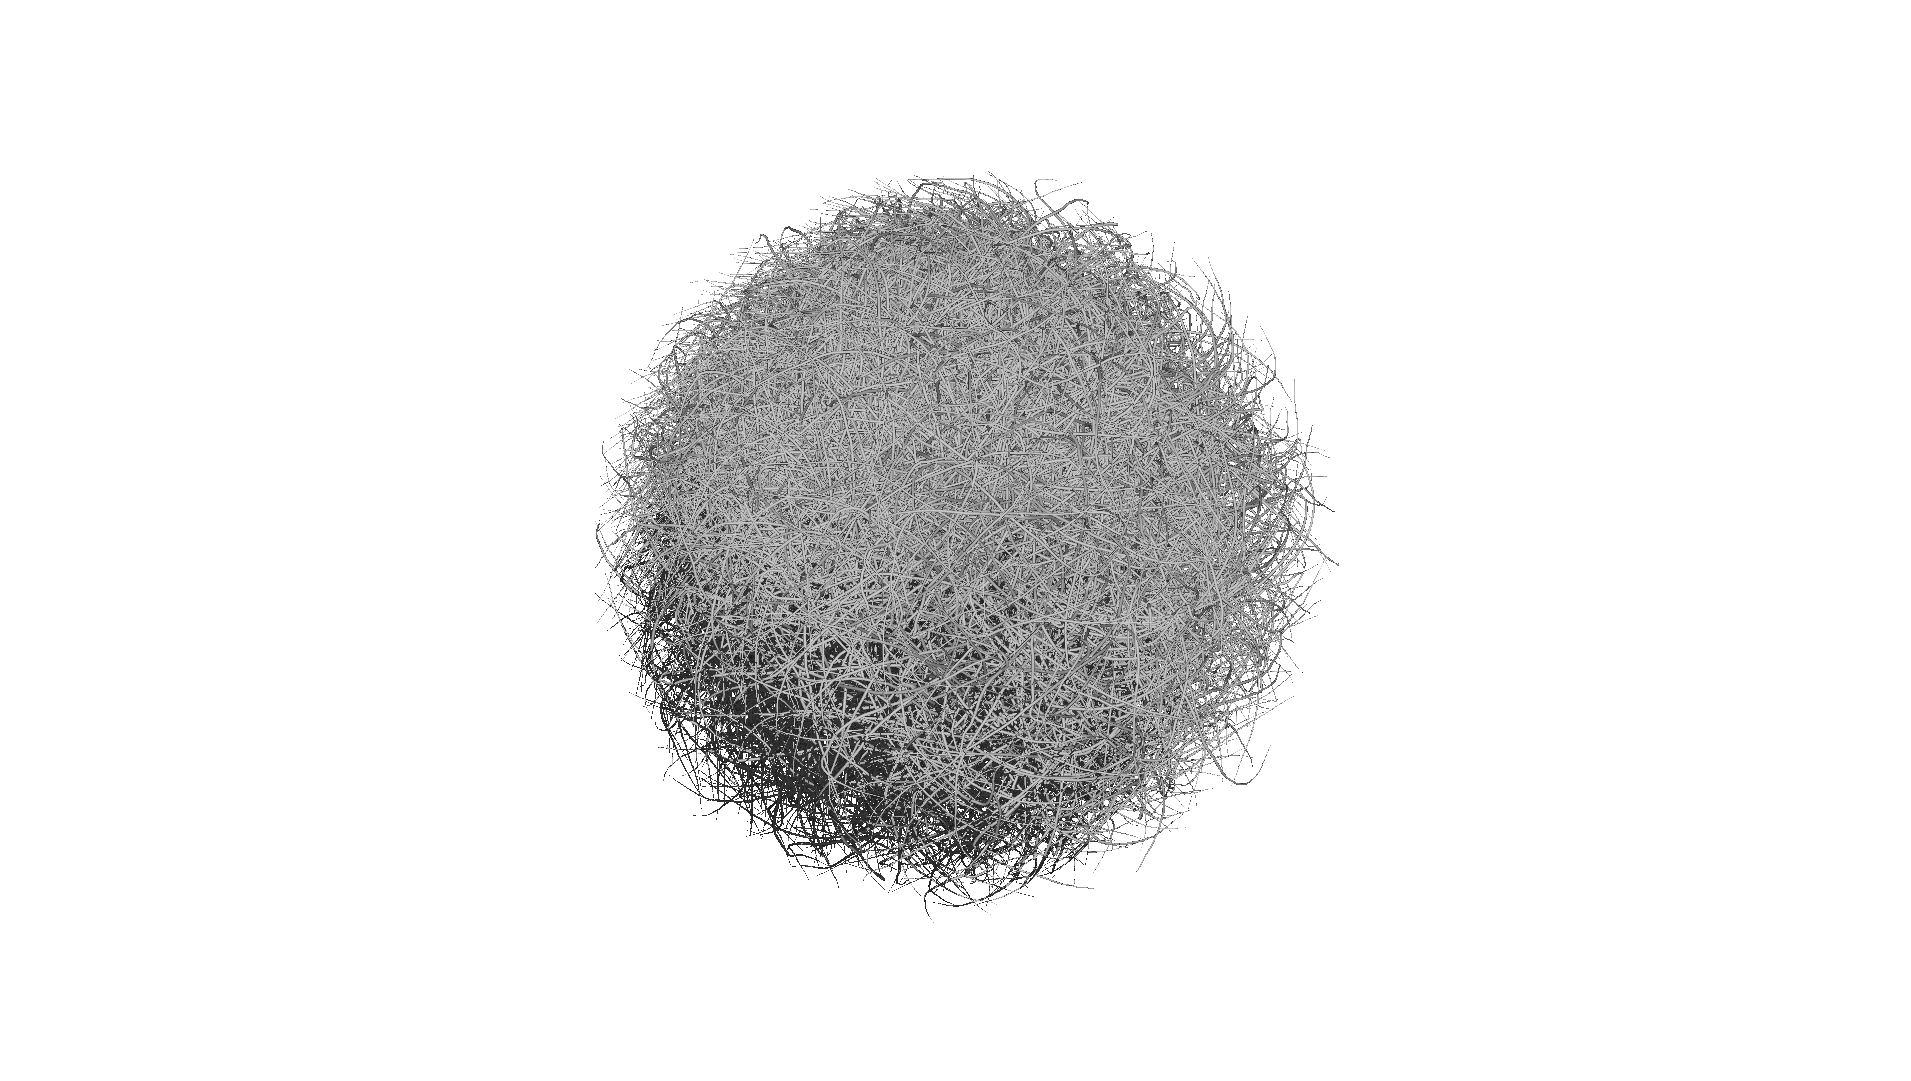
\includegraphics[width=0.75\textwidth]{figuras/hairball.png}
  \caption{Hairball3D model used during our experiments}
  \label{hairball-screenshot}
\end{figure}
In order to better gauge how these scene sizes compare, we have plotted them in graph \ref{scenes-geometry-graph}.

\begin{figure}[hbt!]
  \centering
  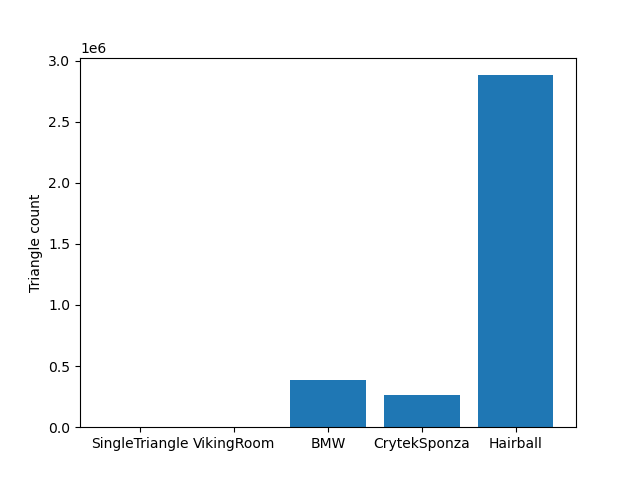
\includegraphics[width=0.75\textwidth]{figuras/scenes-geometry.png}
  \caption{Triangle count of each scene used to test both renderers. We can see how there are orders of magnitude of difference every two of them.}
  \label{scenes-geometry-graph}
\end{figure}

After testing these models we countered some discrepancies with the Acceleration Structure Build Times we expected for each of them. This can be seen in more detail in the Results chapter. We added some extra models for further testing. Their features can be seen in table \ref{extra-scenes-geometry-table} and their triangle counts is graphically compared in plot \ref{extra-scenes-geometry-graph}

\begin{center}
  \begin{tabular}{ | m{3cm} | m{3cm}| m{3cm}|m{3cm} |}
  \hline
  Model name& Triangles& Vertices& Texture size\\
  \hline
    Human& 25422& 29708& 0\\
  \hline
    ISCV2& 383511& 193212& 0\\
  \hline
    Gallery& 998831& 499314& 0\\
  \label{extra-scenes-geometry-table}
\end{tabular}
  % \caption{Scenes that will be used to test the ray tracing libraries compared in this work. We have selected a single 3D model from each order of magnitude in terms of size.}
\end{center}

\begin{figure}[hbt!]
  \centering
  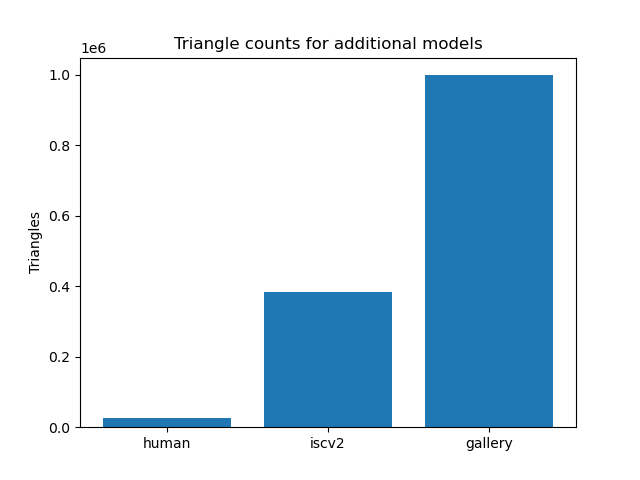
\includegraphics[width=0.75\textwidth]{figuras/extra-scenes-geometry.png}
  \caption{Triangle count of the extra scenes used to further test acceleration structure build times.}
  \label{extra-scenes-geometry-graph}
\end{figure}

Finally, we considered it will be of use compare how each library performed in different hardware configurations. We gathered all the available hardware compatible with GPU accelerated ray tracing, and used it to run the same experiments. This hardware is summarized in table \ref{pc-specs-table}. This will not only allow us to check how different GPUs handle the same workload, but also how they do it inside a virtualized environment: the Intel Core i9 machine is not running the software in bare metal, but rather virtualizing Windows under \textit{QEMU}.

\begin{center}
  \begin{tabular}{ | m{5cm} | m{3.5cm}| m{2cm}|m{4cm} |}
  \hline
  CPU& GPU& RAM& OS\\
  \hline
    Intel Core i7-12700K, 3.60 GHz& Nvidia GeForce RTX 3070& 16 GB& Windows 11, 64 bit\\ % Paco
  \hline
    AMD Ryzen 5 3600 3.6GHz BOX& Nvidia GeForce RTX 2070 Super& 16 GB& Windows 10, 64 bit\\ % Mine
  \hline
    Intel Core i5-9600K, 3.7GHz& Nvidia GeForce RTX 3060 Ti& 16 GB& Windows 10, 64 bit\\ % Juan Carlos
  \hline
    Intel Core i9-9900K (12/16 cores), 3.6GHz& Nvidia GeForce RTX 3080& 16 GB& Windows 10, 64 bit\\ % Roobre
  \hline
    Intel Core i7 10th gen& Nvidia GeForce RTX 3080& 32GB& Windows 10, 64 bit\\ % Naru
  \hline
    AMD Ryzen 7 3800x, 3.9GHz& Nvidia GeForce RTX 2070 Super& 64GB& Windows 11, 64 bit\\ % Jesus
  \hline
    Intel Core i9-12900F& Nvidia GeForce RTX 2060& 32GB& Windows 10, 64 bit\\ % Adrian
  \label{pc-specs-table}
\end{tabular}
  % \caption{Hardware information of the different PCs we managed to run our tests on.}
\end{center}
